\chapter{The Invitation to the Banquet (19:1--19:21)}

Revelation 19 brings us before two very different banquets. The first is the wedding supper\index{wedding supper of the Lamb} of the Lamb\index{Lamb, the}: “Blessed are those who are invited to the wedding supper of the Lamb.” The bride\index{bride of the Lamb} has made herself ready, and heaven resounds with praise. This is the feast of the Lamb and His people, a celebration of salvation, joy, and eternal fellowship.

The second is “the great banquet\index{great banquet of God} of God.” Here, the birds of the sky are summoned to feast upon the flesh of those who have set themselves against God. It is a dreadful counterpart to the wedding supper\index{wedding supper of the Lamb}—a vision of judgment\index{judgment} upon the enemies of the Lord.

Then Christ appears, riding upon a white horse\index{white horse}. He is called “Faithful and True.” In righteousness He judges and wages war, overthrowing the beast\index{beast} and the false prophet\index{false prophet}. The Christ whom the world once rejected and persecuted\index{persecution} now reveals His glory\index{glory} in full. Before Him, every power that opposes God is brought to nothing.

Even today, the Lamb extends His invitation. May we receive His grace\index{grace} by faith, follow Him with steadfast hearts, and make ourselves ready to welcome the King who is coming again.

\section{The Wedding Supper of the Lamb}\index{wedding supper of the Lamb}\index{Lamb, the}

\begin{ScriptureBox2}{Count how many times ``Hallelujah'' appears. Why does the multitude praise God, and what is the bride given to wear?}

\item[19:1] After this I heard what sounded like the roar of a great multitude in heaven shouting:\\
\hspace*{1em}``Hallelujah!\\
\hspace*{1em}Salvation and glory and power belong to our God,

\item[19:2] \hspace*{2em}for true and just are his judgments.\\
\hspace*{1em}He has condemned the great prostitute\\
\hspace*{2em}who corrupted the earth by her adulteries.\\
\hspace*{1em}He has avenged on her the blood of his servants.''

\item[19:3] And again they shouted:\\
\hspace*{1em}``Hallelujah!\\
\hspace*{1em}The smoke from her goes up for ever and ever.''

\item[19:4] The twenty-four elders and the four living creatures fell down and worshiped God, who was seated on the throne. And they cried:\\
\hspace*{1em}``Amen, Hallelujah!''

\item[19:5] Then a voice came from the throne, saying:\\
\hspace*{1em}``Praise our God,\\
\hspace*{2em}all you his servants,\\
\hspace*{1em}you who fear him,\\
\hspace*{2em}both great and small!''

\item[19:6] Then I heard what sounded like a great multitude, like the roar of rushing waters and like loud peals of thunder, shouting:\\
\hspace*{1em}``Hallelujah!\\
\hspace*{2em}For our Lord God Almighty reigns.

\item[19:7] \hspace*{1em}Let us rejoice and be glad\\
\hspace*{2em}and give him glory!\\
\hspace*{1em}For the wedding of the Lamb has come,\\
\hspace*{2em}and his bride has made herself ready.

\item[19:8] \hspace*{1em}Fine linen, bright and clean,\\
\hspace*{2em}was given her to wear.''\\
(Fine linen stands for the righteous acts of God's holy people.)

\item[19:9] Then the angel said to me, ``Write this: Blessed are those who are invited to the wedding supper of the Lamb!'' And he added, ``These are the true words of God.''

\item[19:10] At this I fell at his feet to worship him. But he said to me, ``Don't do that! I am a fellow servant with you and with your brothers and sisters who hold to the testimony of Jesus. Worship God! For it is the Spirit of prophecy who bears testimony to Jesus.''

\end{ScriptureBox2}

The great multitude\index{great multitude} in heaven praises God because His judgments are true and righteous. His justice has been fully revealed, and heaven responds with worship\index{worship}. Among those whose long-awaited vindication is now proclaimed are the martyrs\index{martyrs} we encountered in Revelation 6:10. Beneath the altar\index{altar}, they had cried out, “How long, Sovereign Lord, holy and true, until you judge the inhabitants of the earth and avenge our blood?”

Their question had risen from the suffering of the faithful, whose lives were taken because of their testimony to God. Now, the heavenly chorus declares that their cries have not been forgotten. God's apparent delay was never indifference, and His silence was never the absence of justice. At the appointed time, He judges evil and vindicates His servants.

The scene then turns from the judgment of Babylon\index{Babylon} to the joy of the Lamb's wedding supper\index{wedding supper of the Lamb}. The bride\index{bride of the Lamb} has made herself ready, clothed in fine linen, bright and clean. Yet even this garment is received by grace. The vision identifies the linen with the righteous deeds of God's holy people: their faithful lives are the fruit of belonging to the Lamb. Their readiness is not a claim to glory apart from Him, but the visible expression of a life redeemed\index{redemption} by His grace.

The angel commands John to write down the blessing: those invited to the wedding supper\index{wedding supper of the Lamb} of the Lamb are blessed indeed. This is God's sure promise. The history of the world does not end with the mourning of Babylon\index{Babylon}'s merchants or the defeat of the saints. It moves toward the joyous fellowship of the Lamb and His redeemed people.

\begin{ReaderQuestion}
Revelation 19:9 declares, “Blessed are those who are invited to the wedding supper of the Lamb.” If we truly believe that we have been invited to this supper, how should that assurance shape the way we live today?
\end{ReaderQuestion}

\section{Christ on the White Horse: King of Kings}\index{King of kings}\index{white horse}

\begin{figure}[htbp]
    \centering
    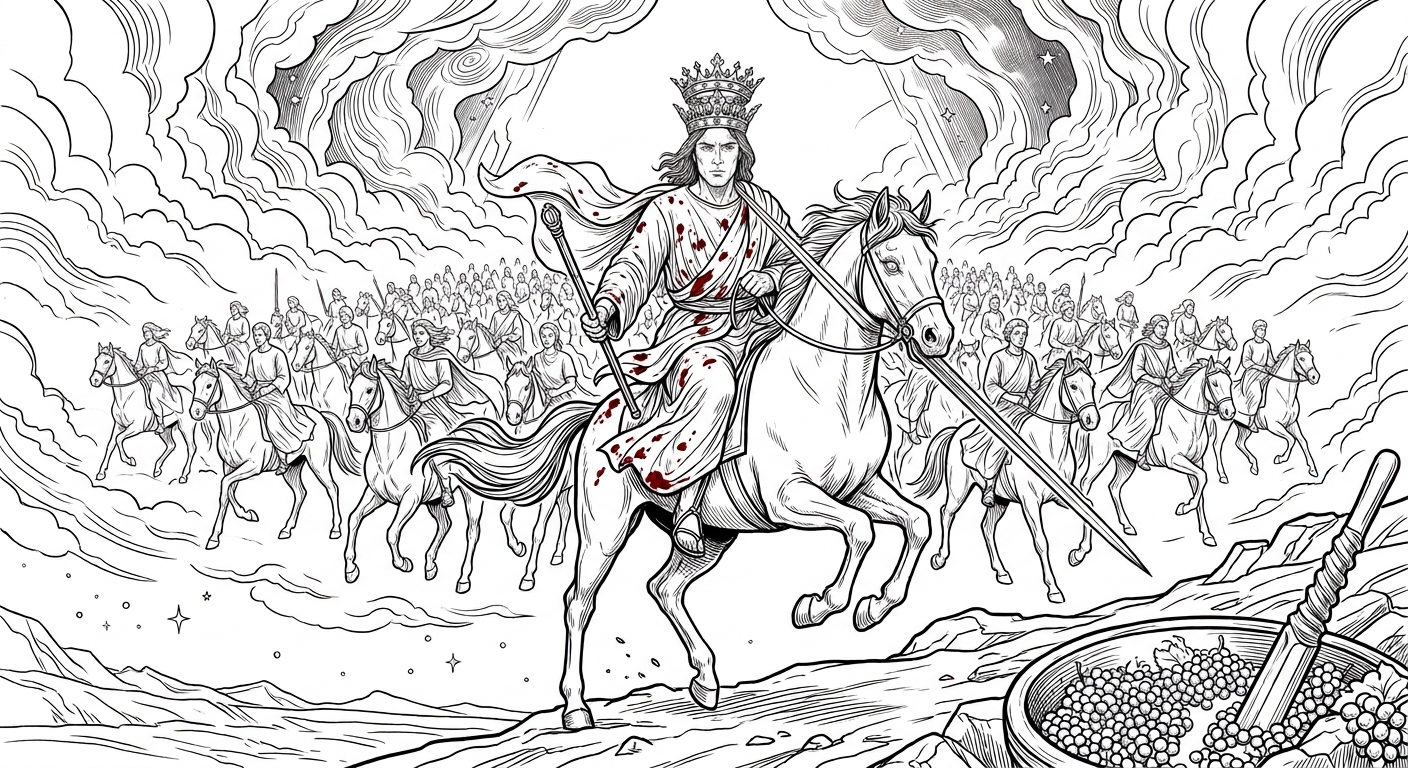
\includegraphics[
    width=1\textwidth,
    trim=0 0 0 0,
    clip]{images/christ_blood_white_horse.jpg}
    %\caption{}
    %\label{}
\end{figure}

\begin{ScriptureBox2}{Circle every name and title given to the rider on the white horse. What is He wearing, and what comes out of His mouth?}

\item[19:11] I saw heaven standing open and there before me was a white horse, whose rider is called Faithful and True. With justice he judges and wages war.

\item[19:12] His eyes are like blazing fire, and on his head are many crowns. He has a name written on him that no one knows but he himself.

\item[19:13] He is dressed in a robe dipped in blood, and his name is the Word of God.

\item[19:14] The armies of heaven were following him, riding on white horses and dressed in fine linen, white and clean.

\item[19:15] Coming out of his mouth is a sharp sword with which to strike down the nations. ``He will rule them with an iron scepter.'' He treads the winepress of the fury of the wrath of God Almighty.
% NIV footnote for 19:15 (omitted; add as \footnote if wanted):
%   ``with an iron scepter'' --- Psalm 2:9
% CHECK NIV: footnote reference quoted from memory; verify against Bible Gateway.

\item[19:16] On his robe and on his thigh he has this name written:\\
\hspace*{1em}\textsc{king of kings and lord of lords.}

\end{ScriptureBox2}

John sees heaven opened and a white horse\index{white horse} appear, with Christ seated upon it. This is not the white horse of Revelation 6. Here, the rider is unmistakably revealed in His royal glory. He is Faithful and True, and He judges and wages war in righteousness. His eyes blaze like fire, and many crowns rest upon His head. His name is the Word of God, and upon His robe and thigh is written the title that declares His supreme authority: King of kings\index{King of kings} and Lord of lords.

His robe is stained with blood. The image evokes the terrible reality of divine judgment, while also recalling the blood through which Christ redeemed His people. The One who comes to judge is the same Lord who gave Himself for sinners. He is not merely another earthly conqueror\index{overcomers}, nor is His victory uncertain. The armies of heaven follow Him, but the decisive power belongs to the King Himself. The sword proceeds from His mouth, signifying the authority of His word to judge the nations.

The world once treated Christ as one who could be rejected, condemned, and crucified. Yet the risen Lord now appears in the majesty that was His all along. The powers of the earth may gather against Him, but no throne\index{throne of God} can rival His throne, no crown can surpass His crown, and no kingdom can withstand His reign. He is the King of kings\index{King of kings} and the Lord of lords.

\begin{ReaderQuestion}
What names and images are used to describe Christ in Revelation 19:11--16? What do the titles “Faithful and True,” “the Word of God,” and “King of kings and Lord of lords” teach you about Him?
\end{ReaderQuestion}

\section{The Great Banquet of God}\index{great banquet of God}

\begin{ScriptureBox2}{Who is invited to the great supper of God? What happens to the beast and the false prophet, and what happens to the rest?}

\item[19:17] And I saw an angel standing in the sun, who cried in a loud voice to all the birds flying in midair, ``Come, gather together for the great supper of God,

\item[19:18] so that you may eat the flesh of kings, generals, and the mighty, of horses and their riders, and the flesh of all people, free and slave, great and small.''

\item[19:19] Then I saw the beast and the kings of the earth and their armies gathered together to wage war against the rider on the horse and his army.

\item[19:20] But the beast was captured, and with it the false prophet who had performed the signs on its behalf. With these signs he had deluded those who had received the mark of the beast and worshiped its image. The two of them were thrown alive into the fiery lake of burning sulfur.

\item[19:21] The rest were killed with the sword coming out of the mouth of the rider on the horse, and all the birds gorged themselves on their flesh.

\end{ScriptureBox2}

In this chapter, Revelation places two banquets side by side: the wedding supper\index{wedding supper of the Lamb} of the Lamb and the great banquet\index{great banquet of God} of God. The contrast could hardly be more striking. The wedding supper celebrates the salvation and joy shared by Christ and His people; the great banquet portrays the final judgment awaiting the powers that oppose God.

An angel standing in the sun calls to the birds flying overhead, summoning them to gather for God's great banquet\index{great banquet of God}. The imagery is stark and unsettling. The kings of the earth, their generals, their warriors, and people of every rank have assembled to wage war against the rider on the white horse\index{white horse} and His army. Yet the outcome is not a contest between equally matched forces. The beast\index{beast} and the false prophet\index{false prophet} are captured and thrown alive into the fiery lake of burning sulfur. The rest are struck down by the sword that comes from the rider's mouth, and the birds gorge themselves on their flesh.

The gathering intended as a show of defiance becomes the scene of utter defeat. The beast, which deceived the nations through its signs and falsehoods, cannot save itself. The earthly kings who placed their confidence in its power cannot rescue it. Their weapons, alliances, and ambitions prove powerless before Christ.

The two banquets therefore reveal two radically different destinies. Those who belong to the Lamb are welcomed into the joy of His eternal kingdom. Those who persist in rebellion against God face His righteous judgment. The invitation of grace and the warning of judgment stand before the reader together. Revelation calls us not merely to observe these visions, but to consider where our own allegiance lies.

The final victory belongs to Christ. The Lamb who was slain\index{Lamb, the!slain} is the King who reigns; the Savior who calls His people to the wedding supper\index{wedding supper of the Lamb} is the Judge before whom every enemy must answer. Blessed are those who belong to Him, who remain faithful to His testimony, and who await His coming with hope.

\begin{ReaderQuestion}
If you were reading Revelation 19 in the midst of suffering, temptation, or uncertainty, which truth would most strengthen your faith: God's true and righteous judgment, the wedding supper of the Lamb, Christ's sovereignty as King of kings, or the Lamb's final victory? Why?
\end{ReaderQuestion}
